%
% Chapter 4
%
\chapter{Implemented Infrastructure} \label{cap:implemented-infrastructure}

This chapter details the infrastructure implemented for the Remote Lab platform, covering the main components, technologies, deployment strategy, and integration between system modules.

\section{Overview}

The Remote Lab platform is designed as a modular, containerized system that enables secure and efficient remote access to laboratory equipment. The infrastructure follows a layered architecture, separating the user interface, backend logic, and hardware integration, and is built with scalability and maintainability in mind.

\begin{figure}[h]
    \begin{center}
        \resizebox{16cm}{!}{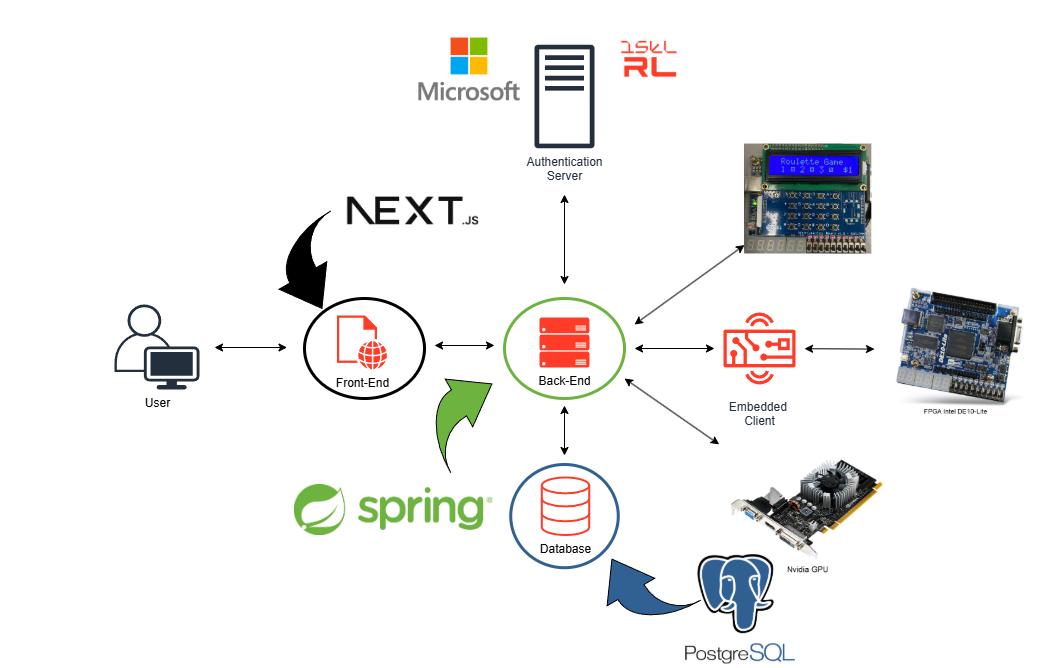
\includegraphics{../img/SystemArchitectureWithTechRL.png}}
    \end{center}
    \caption{System Architecture Overview}
    \label{fig:system-architecture}
\end{figure}

\section{Project Structure}

The Remote Lab project is organized into several main directories, each of which is managed as a GitHub submodule. This approach allows for independent development, versioning, and access control of each core component, supporting both modularity and security. The use of submodules also facilitates collaboration among different teams and ensures that sensitive information is handled appropriately.

The main submodules of the project are:

\begin{itemize}
    \item \textbf{api/} -- Contains the backend source code, implemented in Kotlin with Spring Boot. This submodule is responsible for business logic, user management and laboratory session control.
    \item \textbf{db/} -- Includes database scripts, supporting the persistence layer of the system.
    \item \textbf{docs/} -- Stores project documentation, including technical reports, user guides, and architectural diagrams.
    \item \textbf{img/} -- Stores project images, including diagrams, screenshots, and other visual representations of the system.
    \item \textbf{nginx/} -- This directory is not a GitHub submodule but it provides Nginx configuration files for reverse proxying, load balancing, and secure access to backend services.
    \item \textbf{private/} -- Dedicated to sensitive files and configurations, such as environment variables and secrets necessary for the secure operation of the system, and specific to our implementation choices. This submodule contains the information and configuration files required to run the project with our selected authentication (login) and database setup, reflecting the particular options chosen for our use case. It is not included directly in the main repository, ensuring that only authorized members have access to confidential information like API keys, external service credentials, and other private data essential for both production and development environments.
    \item \textbf{website/} -- Holds the frontend web application, built with Next.js (React). This submodule provides the user interface for laboratory access, scheduling, and management.
    \item \textbf{wiki/} -- Stores the GitHub Wiki pages, including the project documentation, deployment instructions, and other relevant information.
\end{itemize}

This modular structure, based on GitHub submodules, allows for independent development, testing, and deployment of each component, supporting both scalability and maintainability. By clearly separating concerns and leveraging best practices such as containerization and secure secret management, the project is well-positioned for collaborative development and future expansion. 

\section{Implementation Details}

Key implementation decisions and details include:

\begin{itemize}
    \item \textbf{Containerization:} All major components (frontend, backend, database) are containerized using Docker, ensuring consistent environments across development and production.
    \item \textbf{Orchestration:} Docker Compose is used to manage multi-container deployments, networking, and environment configuration.
    \item \textbf{Backend:} The backend uses JDBI for type-safe database access and is configured via environment variables for flexibility and security.
    \item \textbf{Frontend:} The frontend is built with Next.js, providing a modern, responsive interface and integrating with the backend via RESTful APIs.
    \item \textbf{Authentication:} Microsoft OAuth (via NextAuth) is used for secure authentication, enabling university login. The system is designed to be flexible, so other OAuth providers or even an internal login mechanism could be used if required.
    \item \textbf{Role-based Access Control:} The system enforces permissions based on user roles, ensuring secure and appropriate access to resources.
    \item \textbf{Hardware Abstraction:} The backend abstracts hardware-specific details, allowing for easy extension to new laboratory equipment.
    \item \textbf{Automation:} The \texttt{start.sh} script automates the bootstrap process, starting all necessary services with a single command.
\end{itemize}

\subsection*{Role-Based Access Control (RBAC)}

The system implements Role-Based Access Control (RBAC) to ensure that users have access only to the resources and actions appropriate for their role. Each authenticated user is assigned a role, such as student, professor, or administrator, which determines their permissions within the platform. 

Roles are enforced both on the backend and frontend. On the backend, endpoints and business logic check the user's role before allowing access to sensitive operations, such as managing laboratory sessions, accessing administrative features, or modifying user data. On the frontend, the user interface dynamically adapts to the user's role, displaying only the features and options relevant to their permissions.

The main roles in the system are:
\begin{itemize}
    \item \textbf{Student:} Can view and book laboratory sessions, access their own session history, and interact with laboratory equipment during their reserved times. Students have access only to features relevant to their participation in laboratory activities.
    \item \textbf{Professor:} In addition to all student permissions, professors can create and manage laboratory sessions, view and manage student participation, and access additional data and reports related to their classes or laboratories.
    \item \textbf{Administrator:} Has full access to all system features, including user management, system configuration, and oversight of all laboratory sessions and resources. Administrators can manage roles, permissions, and perform maintenance or troubleshooting tasks across the platform.
\end{itemize}

This approach provides a secure and flexible way to manage access, making it easy to introduce new roles or adjust permissions as the platform evolves. The RBAC system is central to maintaining the integrity and security of the Remote Lab environment.

These choices ensure the platform is robust, extensible, and easy to deploy or develop locally.

In addition, the web application allows users to view and interact with the platform as if they had a lower role than their own. This feature is particularly useful for testing, support, and understanding the user experience from different perspectives. For example, an administrator or professor can switch to a student view to verify permissions, troubleshoot issues, or provide guidance, without needing to log in as a different user. 

\section{Database}
Database

\section{Web API}
Web API

\section{Web Application}
Web App

\section{Deployment}

\section{Technologies Used}

\begin{itemize}
    \item \textbf{Frontend:} Implemented with Next.js (React framework), providing a modern, responsive web interface for users to interact with laboratories, schedule sessions, and control hardware.
    \item \textbf{Backend:} Developed in Kotlin using Spring Boot, exposing RESTful APIs for user management, authentication, laboratory session control, and business logic enforcement.
    \item \textbf{Database:} PostgreSQL is used to persist user data, session information, access logs, and configuration settings.
    \item \textbf{ORM/Database Access:} JDBI is used for type-safe, modular database access in the backend.
    \item \textbf{Authentication:} Microsoft OAuth via NextAuth is used for user authentication, supporting multiple roles (student, professor, administrator).
    \item \textbf{Containerization:} Docker is used to containerize all major components (frontend, backend, database), ensuring consistent deployment across environments.
    \item \textbf{Orchestration:} Docker Compose manages multi-container deployment, networking, and environment configuration.
\end{itemize}

\section{System Components}

\begin{itemize}
    \item \textbf{Web Application (Frontend):} Provides dashboards, laboratory access, real-time hardware monitoring, and session management. Built with Next.js and deployed as a Docker container.
    \item \textbf{API Server (Backend):} Handles authentication, authorization, laboratory and user management, and hardware abstraction. Built with Kotlin and Spring Boot, also containerized.
    \item \textbf{Database:} PostgreSQL instance running in a Docker container, with persistent storage volumes.
    \item \textbf{Hardware Abstraction Layer:} Backend modules abstract hardware-specific details, exposing unified interfaces for laboratory equipment control.
\end{itemize}

\section{Deployment Architecture}

The system is deployed using Docker Compose, which defines and manages the following services:

\begin{itemize}
    \item \textbf{db:} PostgreSQL database container, with health checks and persistent volumes.
    \item \textbf{api:} Backend API container, built from the Kotlin/Spring Boot project, depending on the database service.
    \item \textbf{website:} Frontend container, built from the Next.js project, depending on the API service.
\end{itemize}

All services are connected via Docker networks to ensure secure and efficient communication. Environment variables and secrets are managed via \texttt{.env} files.

\section{Build and CI/CD}

\begin{itemize}
    \item \textbf{Gradle:} Used for building and managing backend dependencies.
    \item \textbf{NPM:} Used for frontend dependency management and builds.
    \item \textbf{Dockerfiles:} Multi-stage builds are used for both backend and frontend to optimize image size and security.
    \item \textbf{GitHub Actions:} (If applicable) Used for continuous integration and automated builds.
\end{itemize}

\section{Notable Implementation Details}

\begin{itemize}
    \item The backend uses JDBI for database access, configured with application-specific requirements.
    \item Environment variables are used to configure database connections and secrets, improving security and flexibility.
    \item The system supports role-based access control, with different permissions for students, professors, and administrators.
    \item The hardware abstraction layer allows for future extension to new types of laboratory equipment.
\end{itemize}

\section{Summary}

The implemented infrastructure leverages modern web technologies, containerization, and modular design to provide a robust, scalable, and maintainable platform for remote laboratory access.